% pdflatex -shell-escape canal.tex → canal.png
\documentclass[tikz,convert,border=10pt]{standalone}
\usetikzlibrary{positioning}
\usetikzlibrary{arrows.meta}
\usepackage[utf8]{inputenc}

\tikzset{
 proceso/.style={
 rectangle,
 draw=black, very thick,
 text width=8em,
 minimum height=3em,
 text centered},
 actor/.style={
 rectangle,
 rounded corners,
 draw=black, very thick,
 text width=6em,
 minimum height=3em,
 text centered}
}

\begin{document}
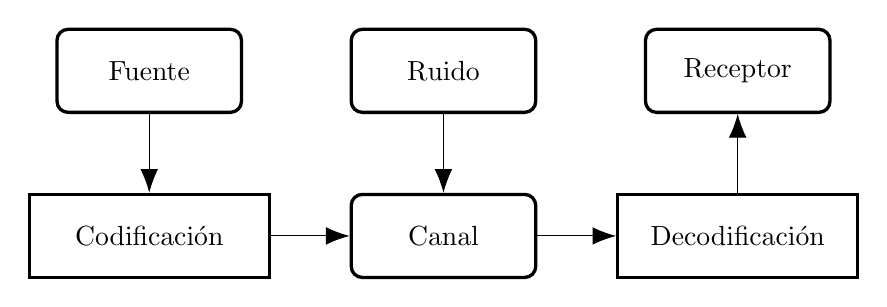
\begin{tikzpicture}
 \node[actor] (canal) {Canal};

 \node[proceso, left = of canal] (cod) {Codificación};
 \node[proceso, right = of canal] (decod) {Decodificación};

 \node[actor, above = of cod] (fuente) {Fuente};
 \node[actor, above = of canal] (ruido) {Ruido};
 \node[actor, above = of decod] (receptor) {Receptor};

 \draw[->,-{Latex[length=3mm]}] (fuente) -- (cod);
 \draw[->,-{Latex[length=3mm]}] (cod) -- (canal);
 \draw[->,-{Latex[length=3mm]}] (canal) -- (decod);
 \draw[->,-{Latex[length=3mm]}] (ruido) -- (canal);
 \draw[->,-{Latex[length=3mm]}] (decod) -- (receptor);
\end{tikzpicture}
\end{document}
